\section{Hyperbolic Equation System}
In the simulatin of partial melting system, 
there arises multidimensional hyperbolic equations systems.
\begin{equation*}
		  \bold{U}_t + \nabla \cdot [F(\bold{U}) - A(\bold{U} \nabla \bold{U})] = 0
\end{equation*}
$\bold{U}$ consists of two variables, average concentration of one species $\bar{c}_1$ and 
average total internal energy $\bar{E}$.
\begin{equation*}
		  \bar{c}_t + \nabla \cdot (\bold{v}_e \bar{c} - \kappa D \nabla \bar{c}) = 0
\end{equation*}
The finite volume discretization can be written as:
$$empty$$

where $\kappa = \frac{\phi_f c_f}{\bar{c}}$ need definition on edge shared between two cells.
\begin{center}
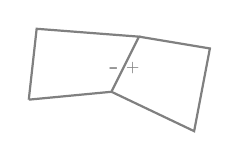
\begin{tikzpicture}
		  \draw[gray,thick] (-0.2,0.1) -- (0.85,0.2) -- (1.2,0.9) -- (-0.1,1) -- (-0.2,0.1);
		  \draw[gray,thick] (0.85,0.2) -- (1.9,-0.3) -- (2.1,0.75) -- (1.2,0.9);
		  \draw[gray] (0.7,0.5) node[anchor=west] {-};
		  \draw[gray,thick] (0.9,0.5) node[anchor=west] {\tiny +};
\end{tikzpicture}
\end{center}
There are two $\kappa$ values defined on both sides of the shared edge.
\begin{equation*}
		  \kappa^{\pm} = \frac{\phi_f c^{\pm}_f}{\bar{c}^{\pm}}
\end{equation*}
where $\phi_f$ has definition on the edge.

\section{A finite volume framework}


